
\section{III - Descente de gradient}
\begin{frame}{III - Descente de gradient}
    \begin{block}{Descente de gradient}
        La Descente de Gradient est un algorithme permettant de trouver un minimum local d'une fonction en convergeant. \\
        Elle est utilisée pour trouver le minimum d'une fonction "coût", évaluant l'erreur entre la valeur de sortie du réseau de neurones et celle attendue: \\
        \begin{center}
            $f : s \mapsto (s - s_{attendue})^2$\\
        \end{center}
        - $s$ la sortie donnée par le modèle \\
        - $s_{attendue}$ la sortie cible. \\
        
    \end{block}
    \begin{exampleblock}{}
        En effet, trouver des paramètres (poids, architecture du réseau, fonction d'activation) permettant d'avoir une erreur nulle revient à résoudre le problème qu'évalue cette fonction coût par rapport aux données d'entrée.
    \end{exampleblock}
\end{frame}


\begin{frame}{III - Descente de gradient}
    \begin{block}{Algorithme du gradient}
        Soit $n \in \mathbb{N}, \varepsilon > 0$. On munit $\mathbb{R}^n$ de son produit scalaire canonique. \\
        Soit $f$ une fonction différentiable de $\mathbb{R}^n \to \mathbb{R}$. \\
        Soit $x_0$ une valeur initiale aléatoire, $t$ le taux d'apprentissage. \\
        Supposons $x_0, \ldots, x_k$ construits. \\
        • Si $\norme{\nabla f(x_k)} \leq \varepsilon$, on s'arrête. \\
        • Sinon on pose $x_{k+1} = x_k - t \nabla f(x_k)$ \\
    \end{block}
    \begin{figure}
        \centering
        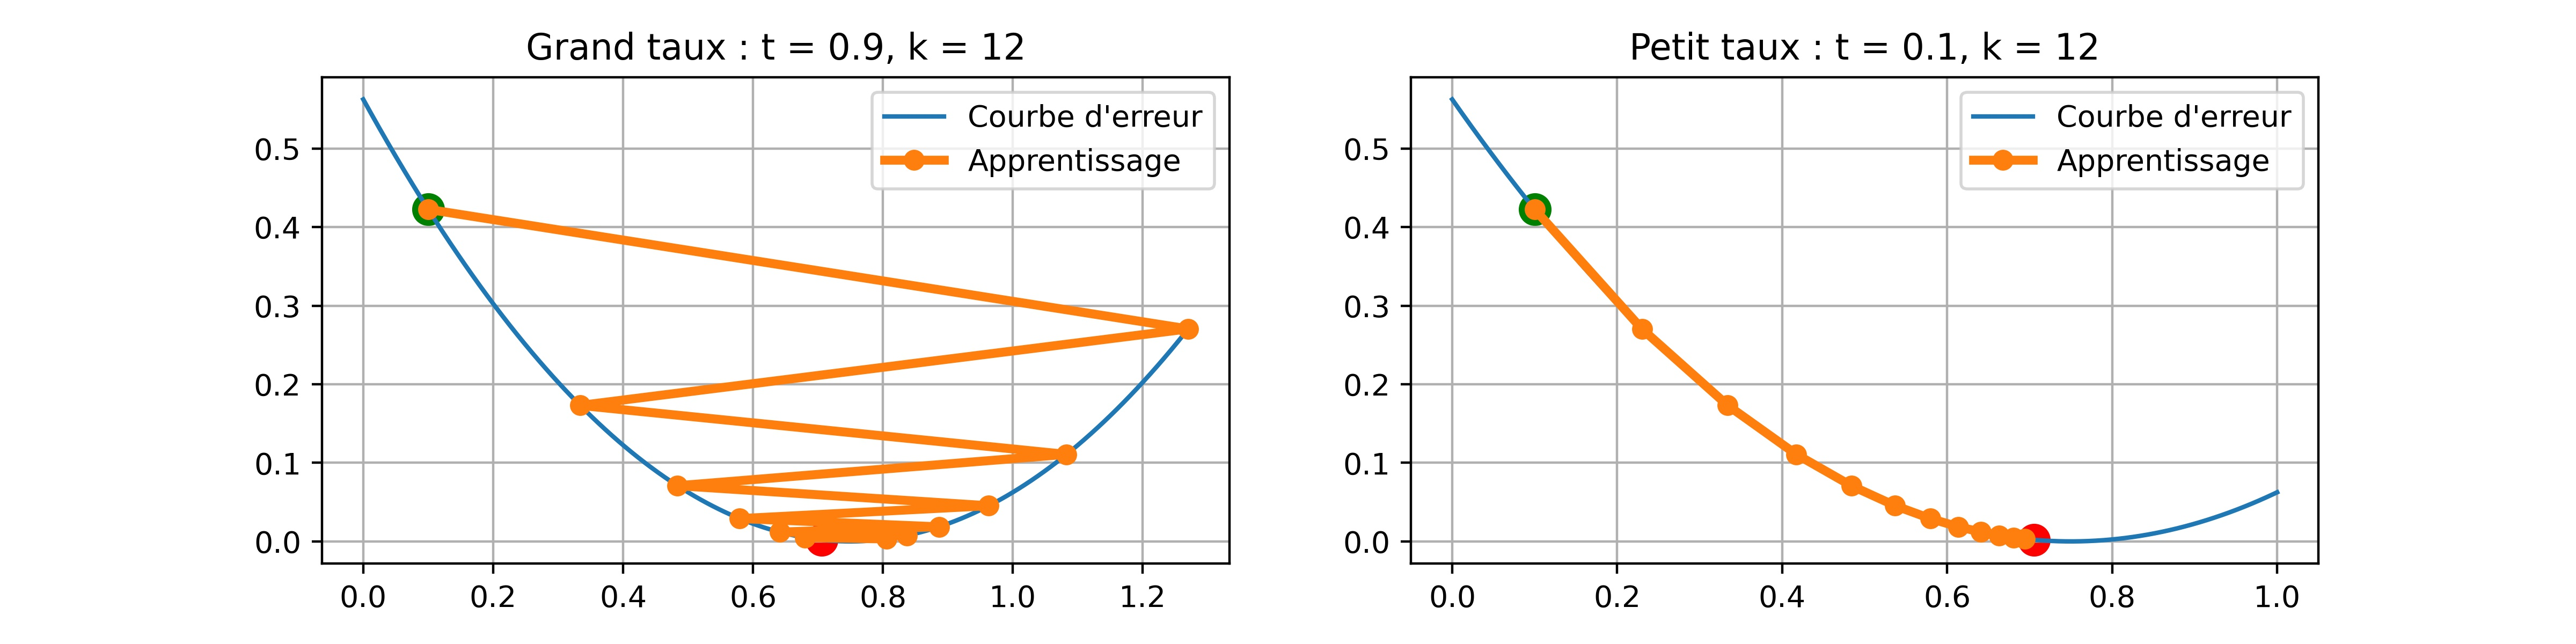
\includegraphics[height=90px]{1-DescenteGradient.jpg}
        \caption{Descente de Gradient pour $f(x) = (x-0.75)^2$; $x_0=0.1$ et $\varepsilon = 0.1$}
    \end{figure}
\end{frame}


\begin{frame}{III - Importance du choix du taux d'apprentissage}
    \begin{exampleblock}{}
        Pour la suite : $f(x) = (x-0.75)^2$ et $x_0=0.1$. \\
    \end{exampleblock}
    \begin{figure}
        \centering
        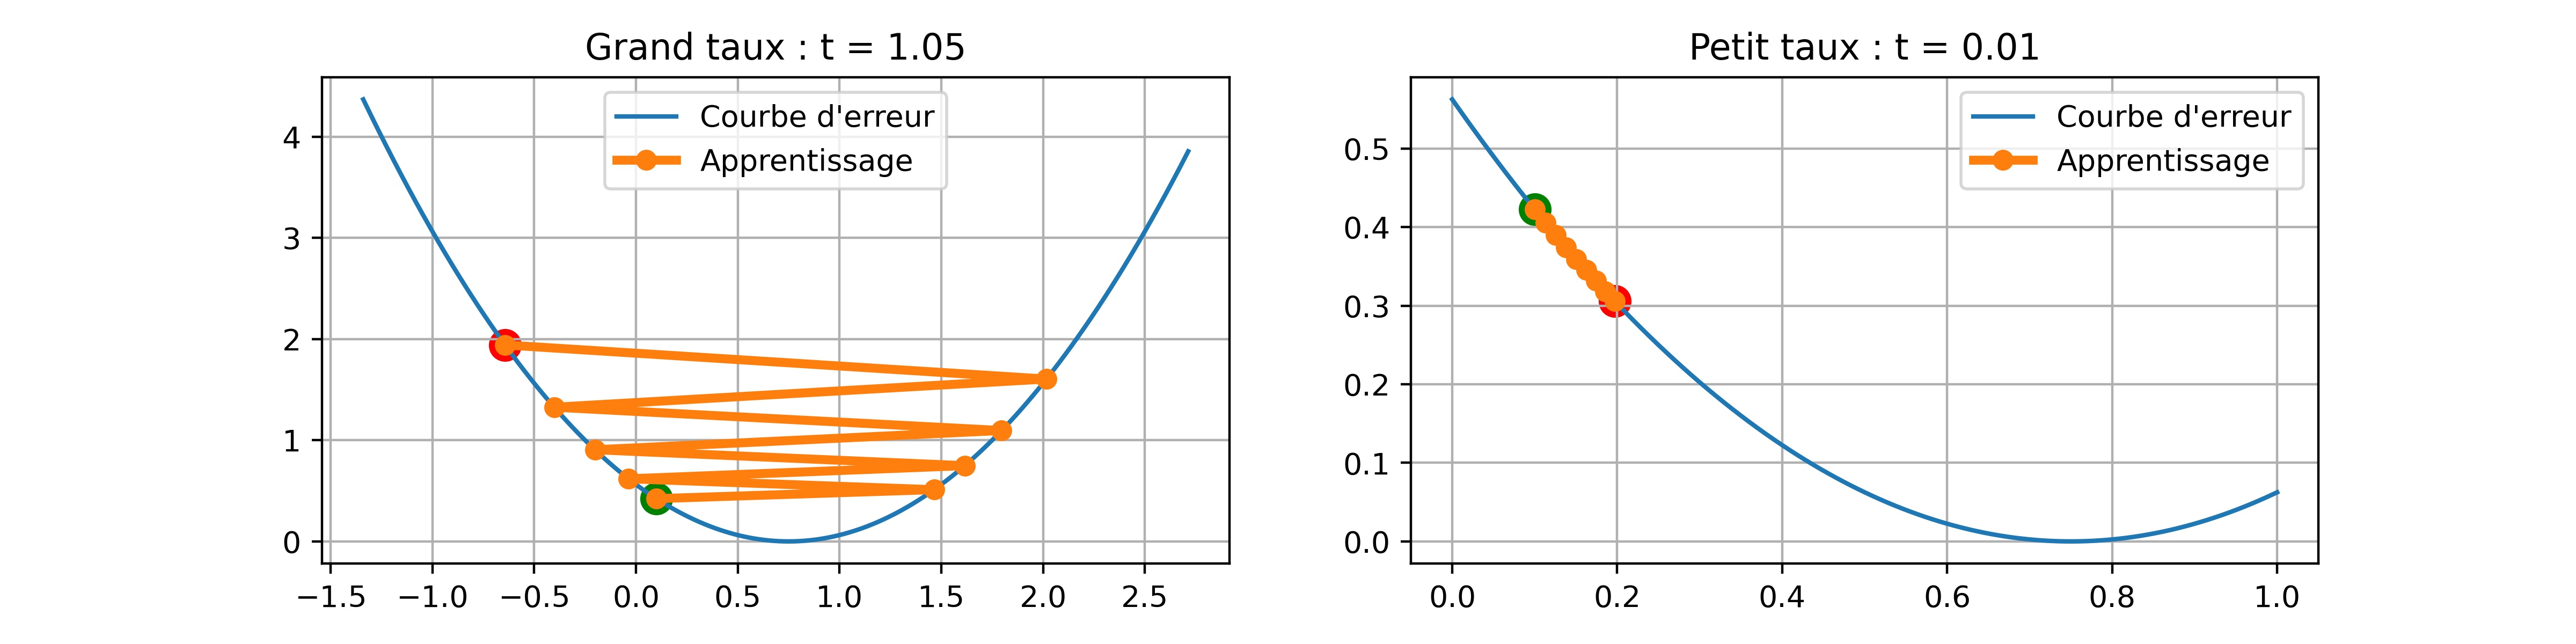
\includegraphics[width=\textwidth]{2-DescenteGradient.jpg}
        \caption{Descente de Gradient on force l'arrêt à $k=8$}
    \end{figure}
    \begin{alertblock}{}
        Les problèmes rencontrés en fonction du choix du taux d'apprentissage : \\
        - trop grand, la descente de gradient diverge \\
        - trop petit , la descente de gradient converge lentement \\
    \end{alertblock}
\end{frame}


\begin{frame}{III - Utilisation du momentum}
    \begin{block}{III - Descente de gradient avec moment}
        $x_0$ aléatoire, momentum $\omega_0 = 0$.
        Supposons $x_0, \ldots, x_k$ et $\omega_0, \ldots, \omega_k$ construits. \\
        • On pose $\omega_{k+1} = \gamma \omega_k + t \nabla f(x_k)$ \\
        • On pose $x_{k+1} = x_k - \omega_{k+1}$
    \end{block}
    \begin{figure}
        \centering
        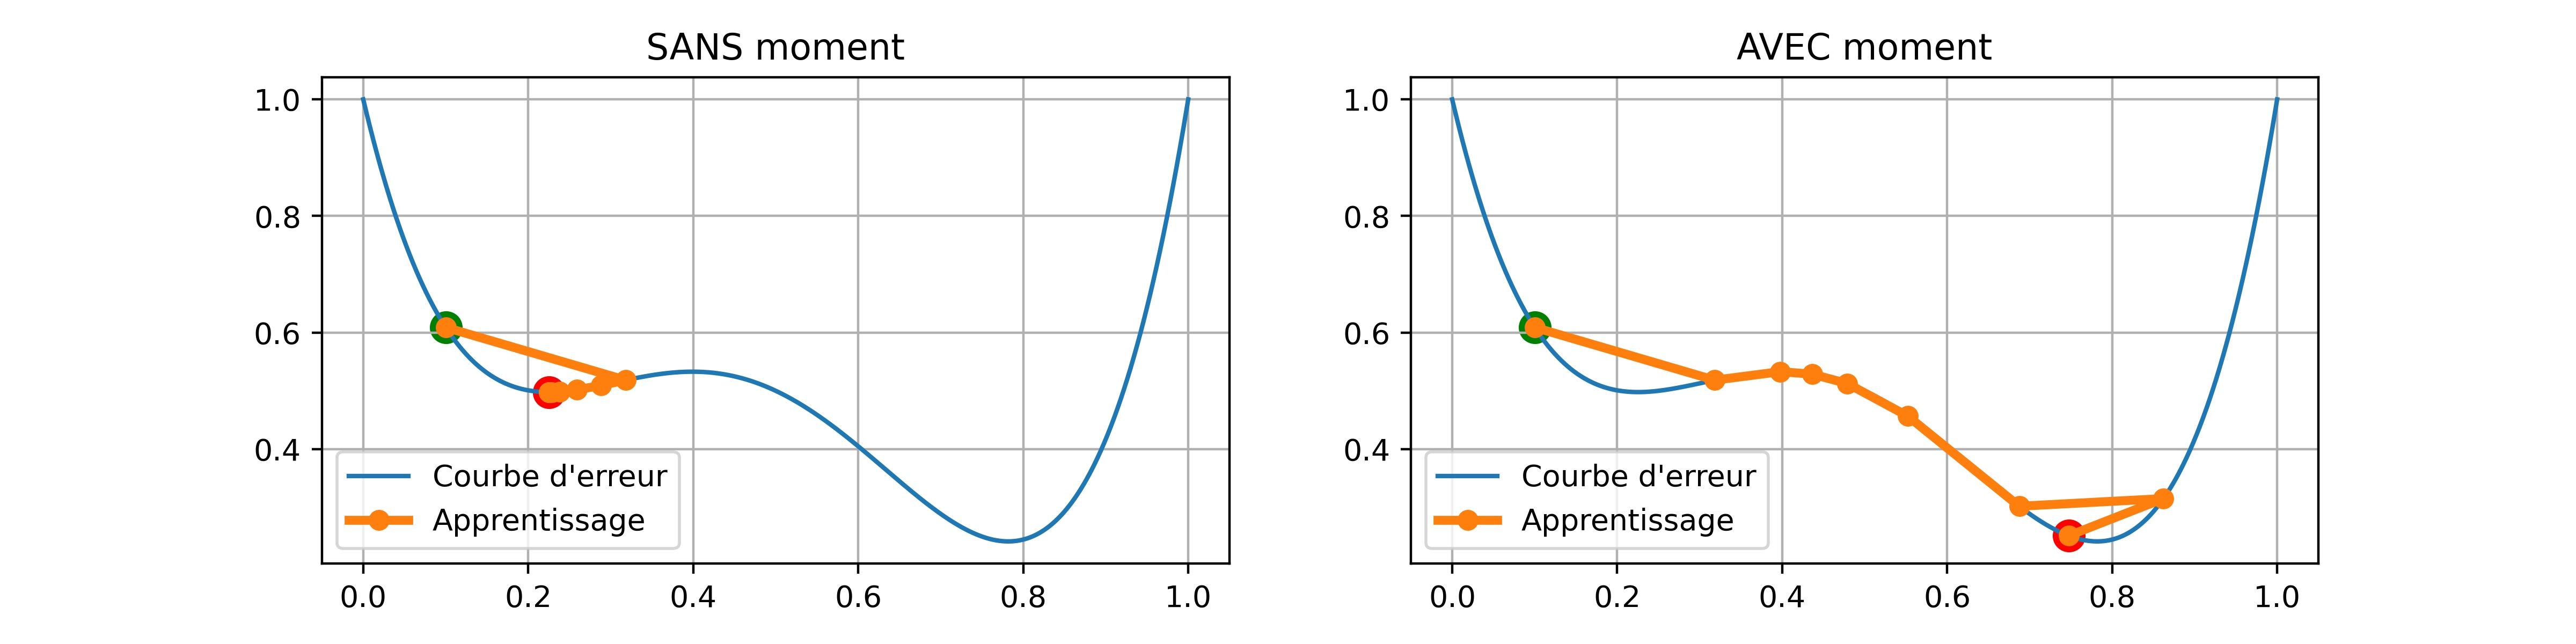
\includegraphics[height=140px]{4-Moment.jpg}
        \caption{Descente de gradient SANS/AVEC momentum où $\gamma = 0.5$, arrêt à $k=4$}
    \end{figure}
\end{frame}


\begin{frame}{III - Utilisation du momentum pour sortir de minima locaux}
    \begin{exampleblock}{Autre avantage}
        Le momentum permet également de s'échapper de minima locaux.        
    \end{exampleblock}
    \begin{figure}
        \centering
        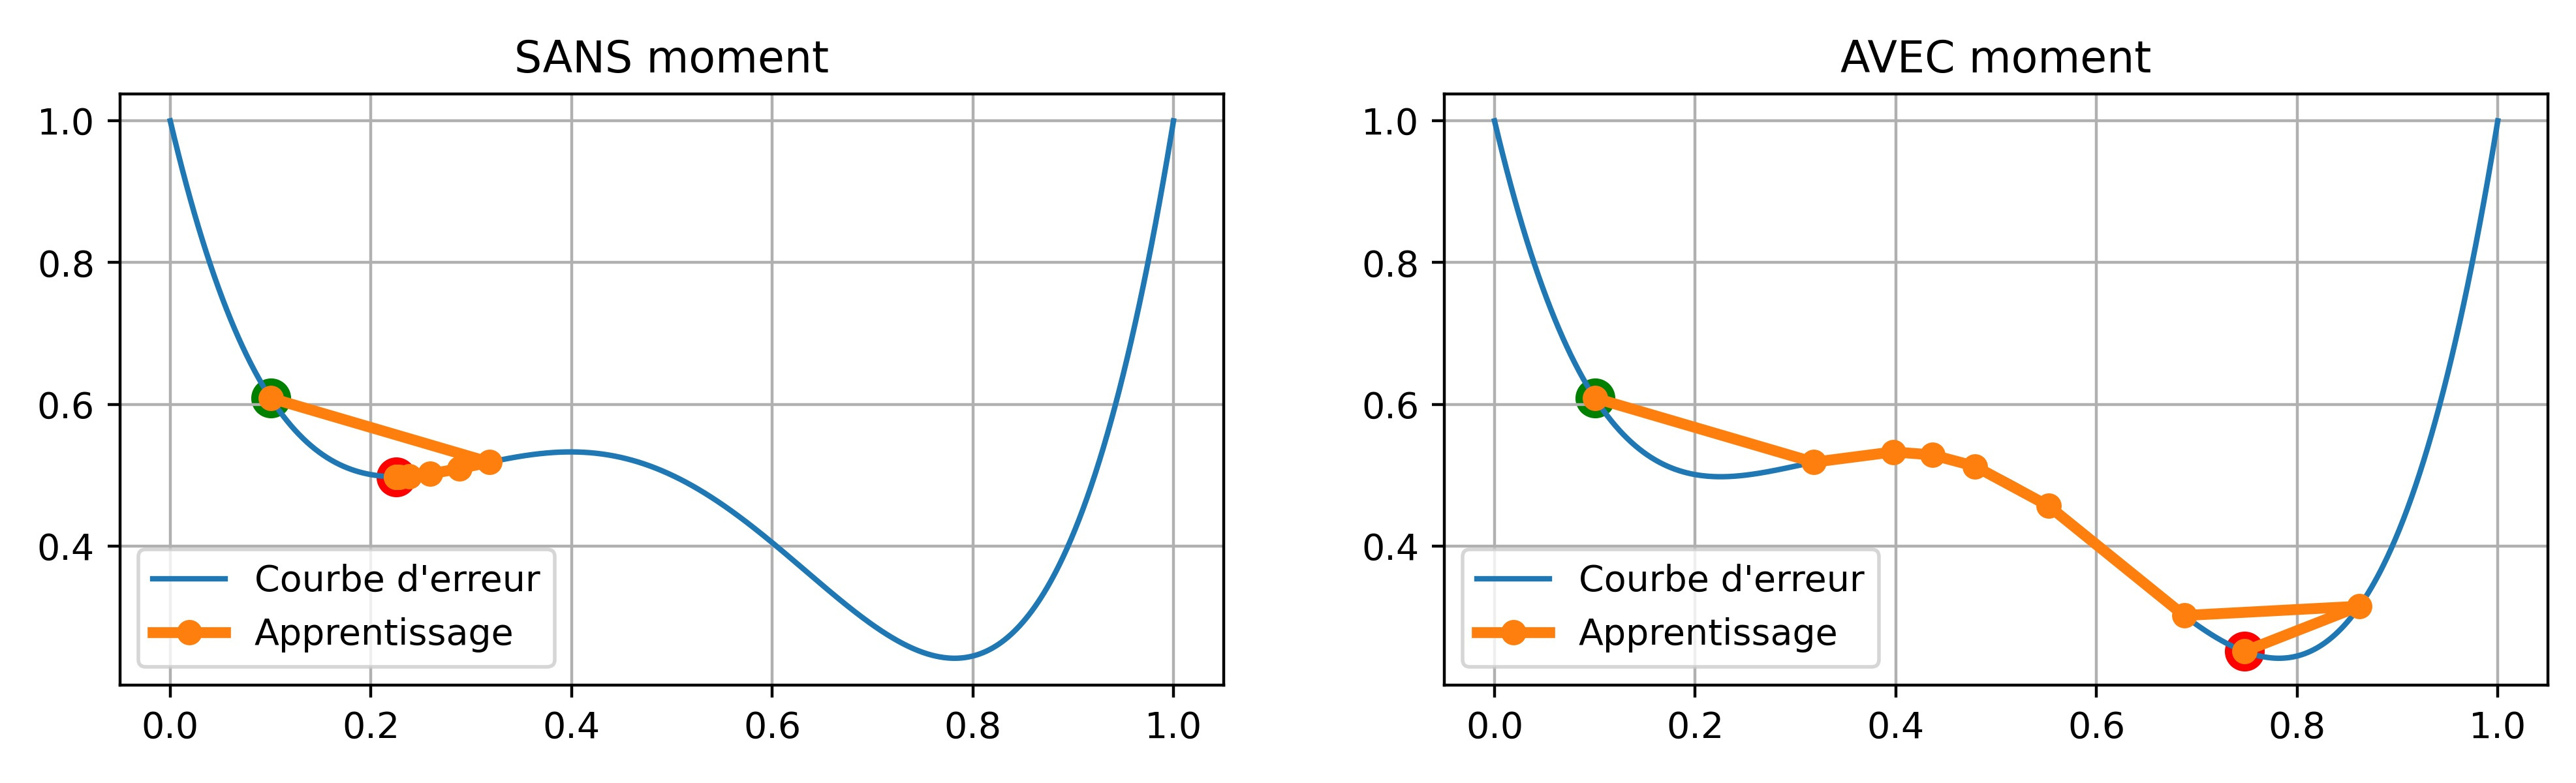
\includegraphics[width=\textwidth, trim=0 10 0 10, clip]{5-Moment.jpg}
        \caption{Descente de gradient SANS/AVEC moment où $\gamma = 0.5$, arrêt à $k=8$}
    \end{figure}
\end{frame}

\begin{frame}{III - Apprentissage stochastique ou par paquet (Batch)}
    \begin{block}{La rétropropagation}
        Ce sont les poids du réseau de neurones qui subissent la descente de gradient.
    \end{block}
    \begin{figure}
        \centering
        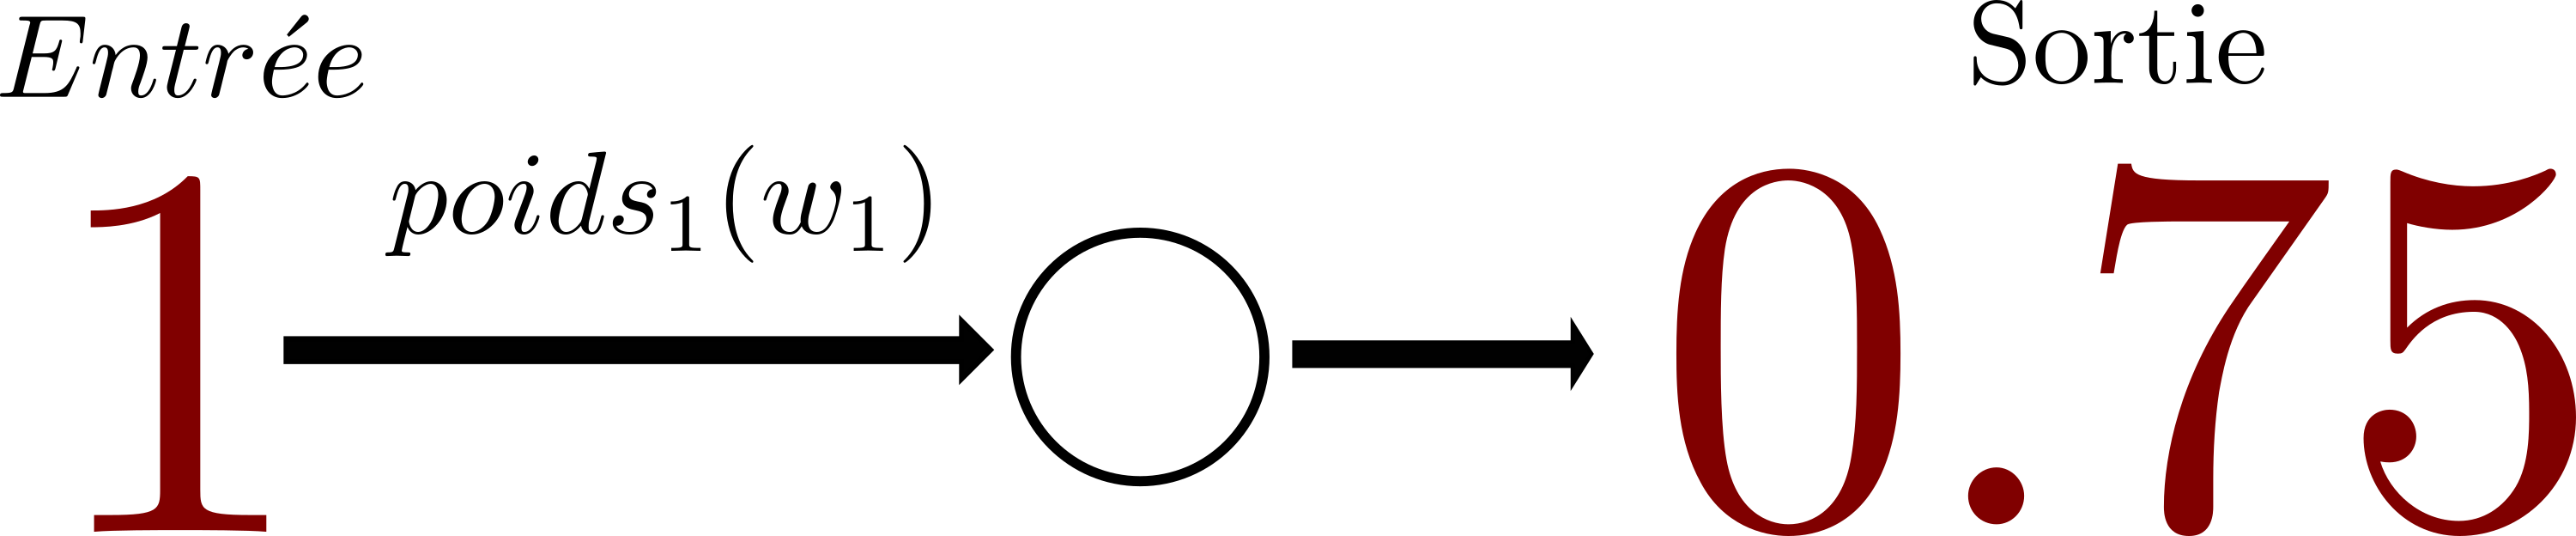
\includegraphics[height=45px]{6-Perceptron.png}
        \caption{Schéma du perceptron linéaire}
    \end{figure}
    \lstinputlisting[language=Python, firstline=15]{3-lineaire.py}
\end{frame}


\begin{frame}{III - Apprentissage stochastique ou par paquet (Batch)}
    \begin{exampleblock}{Problème d'imprécision des données}
        Il faut prendre en compte le fait que les données d'apprentissage ne sont pas toujours exactes. \\
        J'ajoute à mes données une marge d'erreur. 
    \end{exampleblock}
    \begin{block}{}
        Il est alors préférable d'entraîner notre réseau sur des paquets de données plutôt que donnée par donnée. 
    \end{block}
    \begin{center}
        \centering
        $
            \left< f
            \left(
            \begin{pmatrix}
                    x_1^{1} & \ldots & x_n^{1} & b      \\
                    \vdots  & \vdots & \vdots  & \vdots \\
                    x_1^{D} & \ldots & x_n^{D} & b
                \end{pmatrix}
            \times
            \begin{pmatrix}
                    w_1    \\
                    \vdots \\
                    w_n    \\
                    w_b
                \end{pmatrix}
            \right) \right>
        $
    \end{center}
\end{frame}


\begin{frame}{III - Apprentissage stochastique ou par paquet (Batch)}
    \begin{figure}
        \centering
        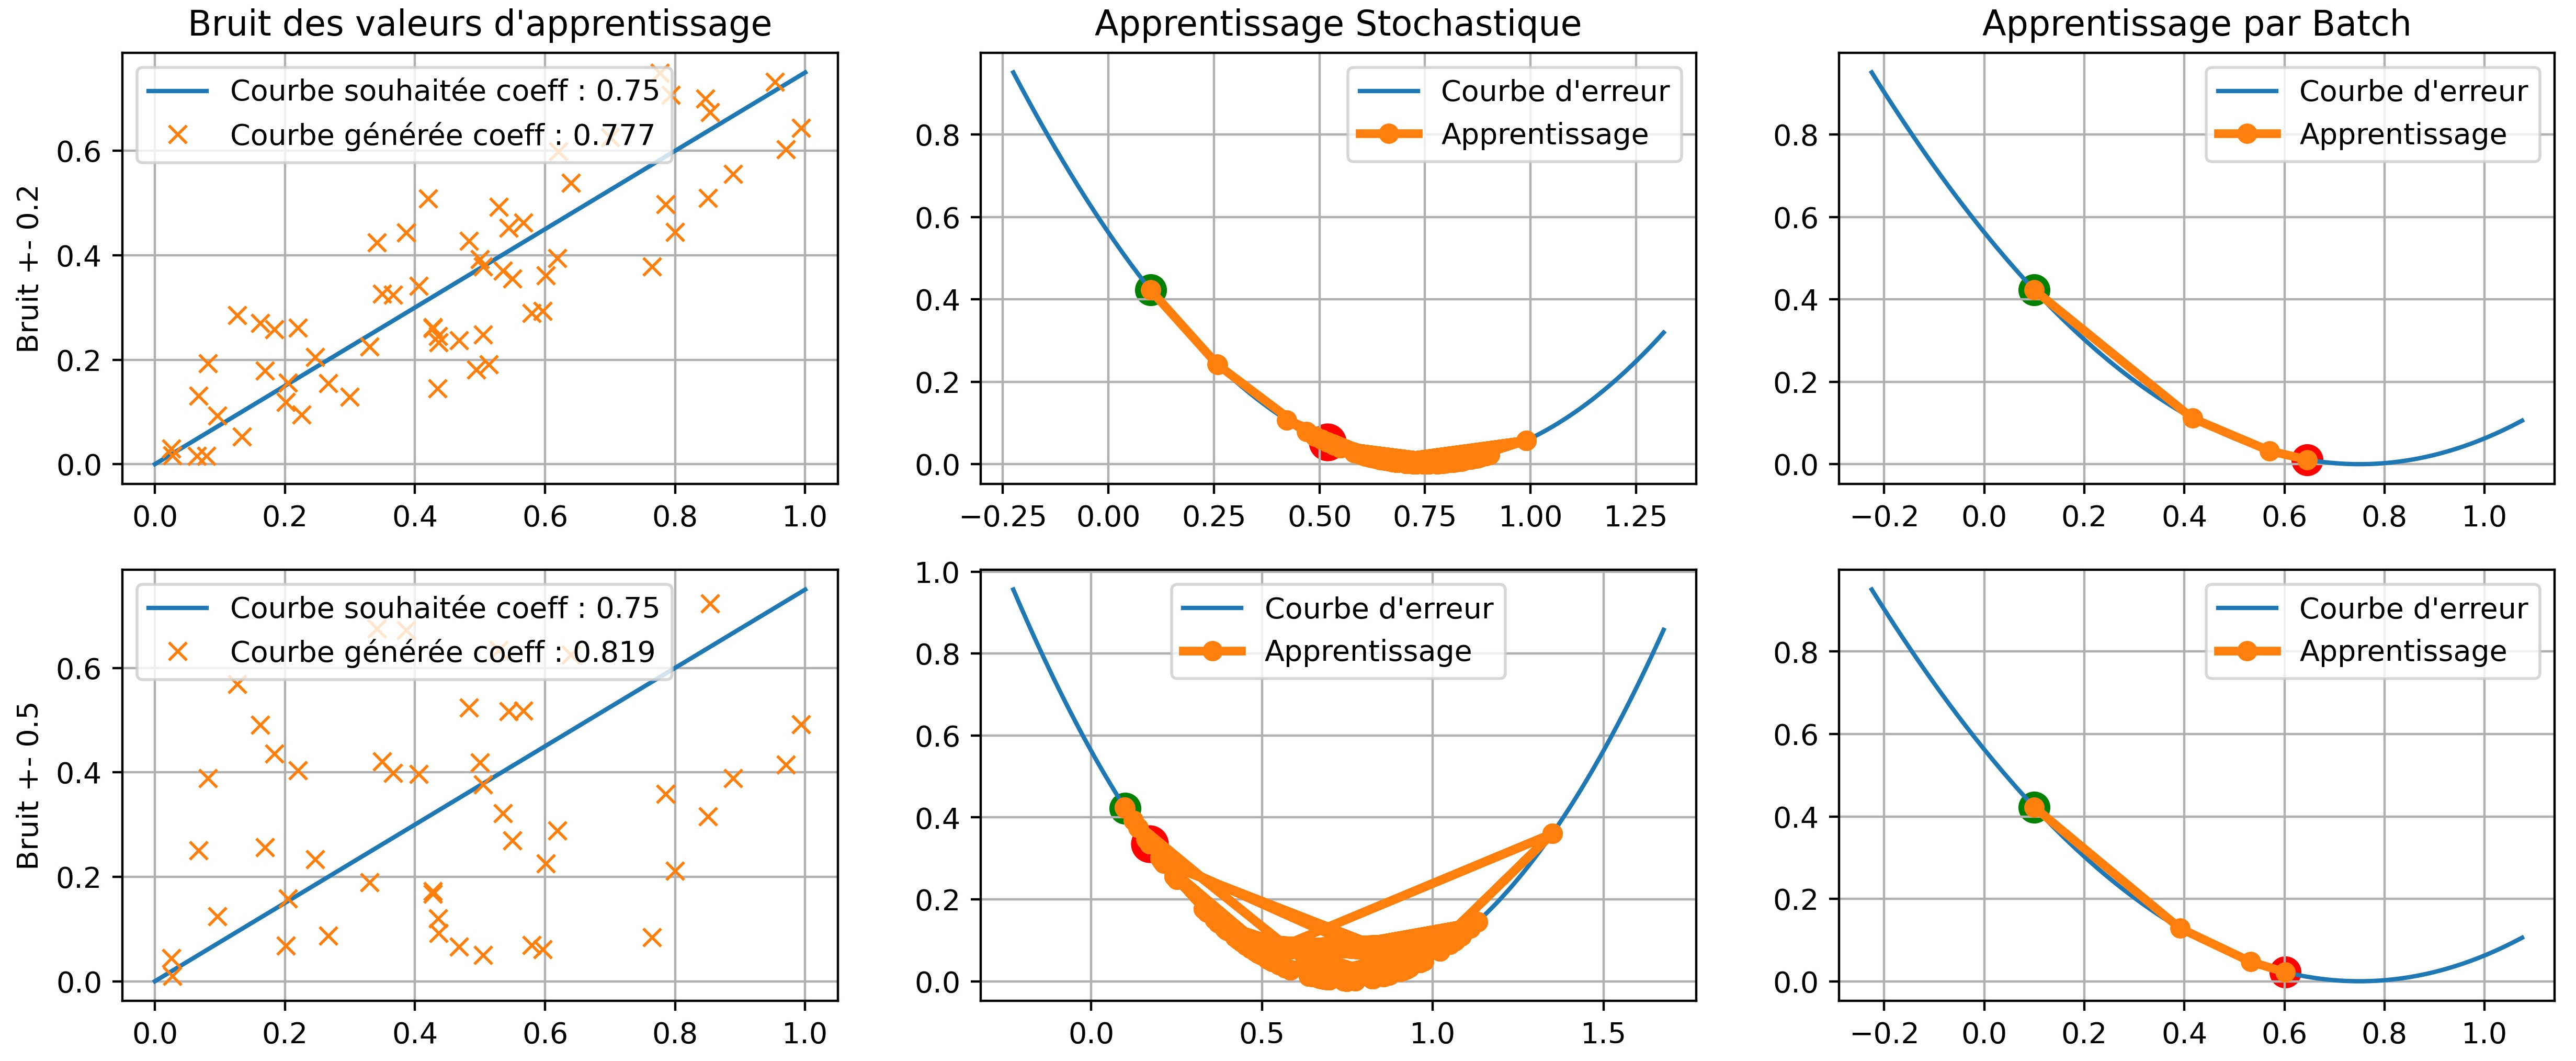
\includegraphics[width=\textwidth]{7-Batch.jpg}
        \caption{Comparaison apprentissage stochastique et par paquet, $f(x) = (x-0.75)^2$}
    \end{figure}
\end{frame}
